\documentclass{zett}
\usepackage{amssymb,amsmath,stmaryrd,mathrsfs}
\usepackage{quiver}
\usepackage{tikz,tikz-cd}
\usepackage{enumitem}
\usepackage{mathtools}
\usepackage{ifmtarg}
\usepackage{braket}
\let\setof\Set
\usepackage{url}
\usepackage{xspace}
\usepackage{mathpartir}
\usepackage{xparse}
\usepackage[activate={true,nocompatibility}]{microtype}
\usepackage[libertine]{newtxmath}

\newcommand{\todo}[1]{{\color{red}\textbf{TODO: }#1}}

% magic
\makeatletter
\let\ea\expandafter

%% Defining commands that are always in math mode.
\def\mdef#1#2{\ea\ea\ea\gdef\ea\ea\noexpand#1\ea{\ea\ensuremath\ea{#2}\xspace}}
\def\alwaysmath#1{\ea\ea\ea\global\ea\ea\ea\let\ea\ea\csname your@#1\endcsname\csname #1\endcsname
  \ea\def\csname #1\endcsname{\ensuremath{\csname your@#1\endcsname}\xspace}}

%% SIMPLE COMMANDS FOR FONTS AND DECORATIONS

\newcount\foreachcount

\def\foreachletter#1#2#3{\foreachcount=#1
  \ea\loop\ea\ea\ea#3\@alph\foreachcount
  \advance\foreachcount by 1
  \ifnum\foreachcount<#2\repeat}

\def\foreachLetter#1#2#3{\foreachcount=#1
  \ea\loop\ea\ea\ea#3\@Alph\foreachcount
  \advance\foreachcount by 1
  \ifnum\foreachcount<#2\repeat}

% Script: \sA is \mathscr{A}
\def\definescr#1{\ea\gdef\csname s#1\endcsname{\ensuremath{\mathscr{#1}}\xspace}}
\foreachLetter{1}{27}{\definescr}
% Calligraphic: \cA is \mathcal{A}
\def\definecal#1{\ea\gdef\csname c#1\endcsname{\ensuremath{\mathcal{#1}}\xspace}}
\foreachLetter{1}{27}{\definecal}
% Bold: \bA is \mathbf{A}
\def\definebold#1{\ea\gdef\csname b#1\endcsname{\ensuremath{\mathbf{#1}}\xspace}}
\foreachLetter{1}{27}{\definebold}
% Blackboard Bold: \dA is \mathbb{A}
\def\definebb#1{\ea\gdef\csname d#1\endcsname{\ensuremath{\mathbb{#1}}\xspace}}
\foreachLetter{1}{27}{\definebb}
% Fraktur: \fa is \mathfrak{a}, except for \fi; \fA is \mathfrak{A}
\def\definefrak#1{\ea\gdef\csname f#1\endcsname{\ensuremath{\mathfrak{#1}}\xspace}}
\foreachletter{1}{9}{\definefrak}
\foreachletter{10}{27}{\definefrak}
\foreachLetter{1}{27}{\definefrak}
% Sans serif: \ia is \mathsf{a}, except for \if and \in and \it
\def\definesf#1{\ea\gdef\csname i#1\endcsname{\ensuremath{\mathsf{#1}}\xspace}}
\foreachletter{1}{6}{\definesf}
\foreachletter{7}{14}{\definesf}
\foreachletter{15}{20}{\definesf}
\foreachletter{21}{27}{\definesf}
\foreachLetter{1}{27}{\definesf}
% Bar: \Abar is \overline{A}, \abar is \overline{a}
\def\definebar#1{\ea\gdef\csname #1bar\endcsname{\ensuremath{\overline{#1}}\xspace}}
\foreachLetter{1}{27}{\definebar}
\foreachletter{1}{8}{\definebar} % \hbar is something else!
\foreachletter{9}{15}{\definebar} % \obar is something else!
\foreachletter{16}{27}{\definebar}
% Tilde: \Atil is \widetilde{A}, \atil is \widetilde{a}
\def\definetil#1{\ea\gdef\csname #1til\endcsname{\ensuremath{\widetilde{#1}}\xspace}}
\foreachLetter{1}{27}{\definetil}
\foreachletter{1}{27}{\definetil}
% Hats: \Ahat is \widehat{A}, \ahat is \widehat{a}
\def\definehat#1{\ea\gdef\csname #1hat\endcsname{\ensuremath{\widehat{#1}}\xspace}}
\foreachLetter{1}{27}{\definehat}
\foreachletter{1}{27}{\definehat}
% Checks: \Achk is \widecheck{A}, \achk is \widecheck{a}
\def\definechk#1{\ea\gdef\csname #1chk\endcsname{\ensuremath{\widecheck{#1}}\xspace}}
\foreachLetter{1}{27}{\definechk}
\foreachletter{1}{27}{\definechk}
% Underline: \uA is \underline{A}, \ua is \underline{a}
\def\defineul#1{\ea\gdef\csname u#1\endcsname{\ensuremath{\underline{#1}}\xspace}}
\foreachLetter{1}{27}{\defineul}
\foreachletter{1}{27}{\defineul}

% Particular commands for typefaces, sometimes with the first letter
% different.
\def\autofmt@n#1\autofmt@end{\mathrm{#1}}
\def\autofmt@b#1\autofmt@end{\mathbf{#1}}
\def\autofmt@d#1#2\autofmt@end{\mathbb{#1}\mathsf{#2}}
\def\autofmt@c#1#2\autofmt@end{\mathcal{#1}\mathit{#2}}
\def\autofmt@s#1#2\autofmt@end{\mathscr{#1}\mathit{#2}}
\def\autofmt@i#1\autofmt@end{\mathsf{#1}}
\def\autofmt@f#1\autofmt@end{\mathfrak{#1}}
% Particular commands for decorations.
\def\autofmt@u#1\autofmt@end{\underline{\smash{\mathsf{#1}}}}
\def\autofmt@U#1\autofmt@end{\underline{\underline{\smash{\mathsf{#1}}}}}
\def\autofmt@h#1\autofmt@end{\widehat{#1}}
\def\autofmt@r#1\autofmt@end{\overline{#1}}
\def\autofmt@t#1\autofmt@end{\widetilde{#1}}
\def\autofmt@k#1\autofmt@end{\check{#1}}

% Defining multi-letter commands.  Use this like so:
% \autodefs{\bSet\cCat\cCAT\kBicat\lProf}
\def\auto@drop#1{}
\def\autodef#1{\ea\ea\ea\@autodef\ea\ea\ea#1\ea\auto@drop\string#1\autodef@end}
\def\@autodef#1#2#3\autodef@end{%
  \ea\def\ea#1\ea{\ea\ensuremath\ea{\csname autofmt@#2\endcsname#3\autofmt@end}\xspace}}
\def\autodefs@end{blarg!}
\def\autodefs#1{\@autodefs#1\autodefs@end}
\def\@autodefs#1{\ifx#1\autodefs@end%
  \def\autodefs@next{}%
  \else%
  \def\autodefs@next{\autodef#1\@autodefs}%
  \fi\autodefs@next}

%% FONTS AND DECORATION FOR GREEK LETTERS

%% the package `mathbbol' gives us blackboard bold greek and numbers,
%% but it does it by redefining \mathbb to use a different font, so that
%% all the other \mathbb letters look different too.  Here we import the
%% font with bb greek and numbers, but assign it a different name,
%% \mathbbb, so as not to replace the usual one.
\DeclareSymbolFont{bbold}{U}{bbold}{m}{n}
\DeclareSymbolFontAlphabet{\mathbbb}{bbold}
\newcommand{\dDelta}{\ensuremath{\mathbbb{\Delta}}\xspace}
\newcommand{\done}{\ensuremath{\mathbbb{1}}\xspace}
\newcommand{\dtwo}{\ensuremath{\mathbbb{2}}\xspace}
\newcommand{\dthree}{\ensuremath{\mathbbb{3}}\xspace}

% greek with bars
\newcommand{\albar}{\ensuremath{\overline{\alpha}}\xspace}
\newcommand{\bebar}{\ensuremath{\overline{\beta}}\xspace}
\newcommand{\gmbar}{\ensuremath{\overline{\gamma}}\xspace}
\newcommand{\debar}{\ensuremath{\overline{\delta}}\xspace}
\newcommand{\phibar}{\ensuremath{\overline{\varphi}}\xspace}
\newcommand{\psibar}{\ensuremath{\overline{\psi}}\xspace}
\newcommand{\xibar}{\ensuremath{\overline{\xi}}\xspace}
\newcommand{\ombar}{\ensuremath{\overline{\omega}}\xspace}

% greek with tildes
\newcommand{\altil}{\ensuremath{\widetilde{\alpha}}\xspace}
\newcommand{\betil}{\ensuremath{\widetilde{\beta}}\xspace}
\newcommand{\gmtil}{\ensuremath{\widetilde{\gamma}}\xspace}
\newcommand{\phitil}{\ensuremath{\widetilde{\varphi}}\xspace}
\newcommand{\psitil}{\ensuremath{\widetilde{\psi}}\xspace}
\newcommand{\xitil}{\ensuremath{\widetilde{\xi}}\xspace}
\newcommand{\omtil}{\ensuremath{\widetilde{\omega}}\xspace}

% MISCELLANEOUS SYMBOLS
\let\del\partial
\mdef\delbar{\overline{\partial}}
\let\sm\wedge
\newcommand{\dd}[1]{\ensuremath{\frac{\partial}{\partial {#1}}}}
\newcommand{\inv}{^{-1}}
\newcommand{\dual}{^{\vee}}
\mdef\hf{\textstyle\frac12 }
\mdef\thrd{\textstyle\frac13 }
\mdef\qtr{\textstyle\frac14 }
\let\meet\wedge
\let\join\vee
\let\dn\downarrow
\newcommand{\op}{^{\mathrm{op}}}
\newcommand{\co}{^{\mathrm{co}}}
\newcommand{\coop}{^{\mathrm{coop}}}
\let\adj\dashv
\let\iso\cong
\let\eqv\simeq
\let\cng\equiv
\mdef\Id{\mathrm{Id}}
\mdef\id{\mathrm{id}}
\alwaysmath{ell}
\alwaysmath{infty}
\let\oo\infty
\def\io{\ensuremath{(\infty,1)}}
\alwaysmath{odot}
\def\frc#1/#2.{\frac{#1}{#2}}   % \frc x^2+1 / x^2-1 .
\mdef\ten{\mathrel{\otimes}}
\let\bigten\bigotimes
\mdef\sqten{\mathrel{\boxtimes}}
\def\lt{<}                      % For iTex compatibility
\def\gt{>}

%%% Blanks (shorthand for lambda abstractions)
\newcommand{\blank}{\mathord{\hspace{1pt}\text{--}\hspace{1pt}}}
%%% Nameless objects
\newcommand{\nameless}{\mathord{\hspace{1pt}\underline{\hspace{1ex}}\hspace{1pt}}}

% Hiragana "yo" for the Yoneda embedding, from https://arxiv.org/abs/1506.08870
\DeclareFontFamily{U}{min}{}
\DeclareFontShape{U}{min}{m}{n}{<-> udmj30}{}
\newcommand{\yon}{\!\text{\usefont{U}{min}{m}{n}\symbol{'210}}\!}

%% Get some new symbols from mathabx, without changing the old ones by
%% importing the package.  Font declarations copied from mathabx.sty:
\DeclareFontFamily{U}{mathb}{\hyphenchar\font45}
\DeclareFontShape{U}{mathb}{m}{n}{
      <5> <6> <7> <8> <9> <10> gen * mathb
      <10.95> mathb10 <12> <14.4> <17.28> <20.74> <24.88> mathb12
      }{}
\DeclareSymbolFont{mathb}{U}{mathb}{m}{n}
\DeclareFontSubstitution{U}{mathb}{m}{n}
\DeclareFontFamily{U}{mathx}{\hyphenchar\font45}
\DeclareFontShape{U}{mathx}{m}{n}{
      <5> <6> <7> <8> <9> <10>
      <10.95> <12> <14.4> <17.28> <20.74> <24.88>
      mathx10
      }{}
\DeclareSymbolFont{mathx}{U}{mathx}{m}{n}
\DeclareFontSubstitution{U}{mathx}{m}{n}
%% And now the symbols we want, copied from mathabx.dcl
\DeclareMathSymbol{\dotplus}       {2}{mathb}{"00}% name to be checked
\DeclareMathSymbol{\dotdiv}        {2}{mathb}{"01}% name to be checked
\DeclareMathSymbol{\dottimes}      {2}{mathb}{"02}% name to be checked
\DeclareMathSymbol{\divdot}        {2}{mathb}{"03}% name to be checked
\DeclareMathSymbol{\udot}          {2}{mathb}{"04}% name to be checked
\DeclareMathSymbol{\square}        {2}{mathb}{"05}% name to be checked
\DeclareMathSymbol{\Asterisk}      {2}{mathb}{"06}
\DeclareMathSymbol{\bigast}        {1}{mathb}{"06}
\DeclareMathSymbol{\coAsterisk}    {2}{mathb}{"07}
\DeclareMathSymbol{\bigcoast}      {1}{mathb}{"07}
\DeclareMathSymbol{\circplus}      {2}{mathb}{"08}% name to be checked
\DeclareMathSymbol{\pluscirc}      {2}{mathb}{"09}% name to be checked
\DeclareMathSymbol{\convolution}   {2}{mathb}{"0A}% name to be checked
\DeclareMathSymbol{\divideontimes} {2}{mathb}{"0B}% name to be checked
\DeclareMathSymbol{\blackdiamond}  {2}{mathb}{"0C}% name to be checked
\DeclareMathSymbol{\sqbullet}      {2}{mathb}{"0D}% name to be checked
\DeclareMathSymbol{\bigstar}       {2}{mathb}{"0E}
\DeclareMathSymbol{\bigvarstar}    {2}{mathb}{"0F}
\DeclareMathSymbol{\corresponds}   {3}{mathb}{"1D}% name to be checked
\DeclareMathSymbol{\boxleft}      {2}{mathb}{"68}
\DeclareMathSymbol{\boxright}     {2}{mathb}{"69}
\DeclareMathSymbol{\boxtop}       {2}{mathb}{"6A}
\DeclareMathSymbol{\boxbot}       {2}{mathb}{"6B}
\DeclareMathSymbol{\updownarrows}          {3}{mathb}{"D6}
\DeclareMathSymbol{\downuparrows}          {3}{mathb}{"D7}
\DeclareMathSymbol{\Lsh}                   {3}{mathb}{"E8}
\DeclareMathSymbol{\Rsh}                   {3}{mathb}{"E9}
\DeclareMathSymbol{\dlsh}                  {3}{mathb}{"EA}
\DeclareMathSymbol{\drsh}                  {3}{mathb}{"EB}
\DeclareMathSymbol{\looparrowdownleft}     {3}{mathb}{"EE}
\DeclareMathSymbol{\looparrowdownright}    {3}{mathb}{"EF}
% \DeclareMathSymbol{\curvearrowleft}        {3}{mathb}{"F0}
% \DeclareMathSymbol{\curvearrowright}       {3}{mathb}{"F1}
\DeclareMathSymbol{\curvearrowleftright}   {3}{mathb}{"F2}
\DeclareMathSymbol{\curvearrowbotleft}     {3}{mathb}{"F3}
\DeclareMathSymbol{\curvearrowbotright}    {3}{mathb}{"F4}
\DeclareMathSymbol{\curvearrowbotleftright}{3}{mathb}{"F5}
% \DeclareMathSymbol{\circlearrowleft}       {3}{mathb}{"F6}
% \DeclareMathSymbol{\circlearrowright}      {3}{mathb}{"F7}
\DeclareMathSymbol{\leftsquigarrow}        {3}{mathb}{"F8}
\DeclareMathSymbol{\rightsquigarrow}       {3}{mathb}{"F9}
\DeclareMathSymbol{\leftrightsquigarrow}   {3}{mathb}{"FA}
\DeclareMathSymbol{\lefttorightarrow}      {3}{mathb}{"FC}
\DeclareMathSymbol{\righttoleftarrow}      {3}{mathb}{"FD}
\DeclareMathSymbol{\uptodownarrow}         {3}{mathb}{"FE}
\DeclareMathSymbol{\downtouparrow}         {3}{mathb}{"FF}
\DeclareMathSymbol{\varhash}       {0}{mathb}{"23}
\DeclareMathSymbol{\sqSubset}       {3}{mathb}{"94}
\DeclareMathSymbol{\sqSupset}       {3}{mathb}{"95}
\DeclareMathSymbol{\nsqSubset}      {3}{mathb}{"96}
\DeclareMathSymbol{\nsqSupset}      {3}{mathb}{"97}
% WIDECHECK
\DeclareMathAccent{\widecheck}    {0}{mathx}{"71}


%% OPERATORS
\DeclareMathOperator\lan{Lan}
\DeclareMathOperator\ran{Ran}
\DeclareMathOperator\colim{colim}
\DeclareMathOperator\coeq{coeq}
\DeclareMathOperator\ob{ob}
\DeclareMathOperator\cod{cod}
\DeclareMathOperator\dom{dom}
\DeclareMathOperator\ev{ev}
\DeclareMathOperator\eq{eq}
\DeclareMathOperator\Tot{Tot}
\DeclareMathOperator\cosk{cosk}
\DeclareMathOperator\sk{sk}
\DeclareMathOperator\img{im}
\DeclareMathOperator\Spec{Spec}
\DeclareMathOperator\Ho{Ho}
\DeclareMathOperator\Aut{Aut}
\DeclareMathOperator\End{End}
\DeclareMathOperator\Hom{Hom}
\DeclareMathOperator\Map{Map}
\DeclareMathOperator\coker{coker}

%% ARROWS
% \to already exists
\newcommand{\too}[1][]{\ensuremath{\overset{#1}{\longrightarrow}}}
\newcommand{\ot}{\ensuremath{\leftarrow}}
\newcommand{\oot}[1][]{\ensuremath{\overset{#1}{\longleftarrow}}}
\let\toot\rightleftarrows
\let\otto\leftrightarrows
\let\Impl\Rightarrow
\let\imp\Rightarrow
\let\toto\rightrightarrows
\let\into\hookrightarrow
\let\xinto\xhookrightarrow
\mdef\we{\overset{\sim}{\longrightarrow}}
\mdef\leftwe{\overset{\sim}{\longleftarrow}}
\let\mono\rightarrowtail
\let\leftmono\leftarrowtail
\let\cof\rightarrowtail
\let\leftcof\leftarrowtail
\let\epi\twoheadrightarrow
\let\leftepi\twoheadleftarrow
\let\fib\twoheadrightarrow
\let\leftfib\twoheadleftarrow
\let\cohto\rightsquigarrow
\let\maps\colon
\newcommand{\spam}{\,:\!}       % \maps for left arrows
\def\acof{\mathrel{\mathrlap{\hspace{3pt}\raisebox{4pt}{$\scriptscriptstyle\sim$}}\mathord{\rightarrowtail}}}

% diagxy redefines \to, along with \toleft, \two, \epi, and \mon.

%% EXTENSIBLE ARROWS
\let\xto\xrightarrow
\let\xot\xleftarrow
% See Voss' Mathmode.tex for instructions on how to create new
% extensible arrows.
\def\rightarrowtailfill@{\arrowfill@{\Yright\joinrel\relbar}\relbar\rightarrow}
\newcommand\xrightarrowtail[2][]{\ext@arrow 0055{\rightarrowtailfill@}{#1}{#2}}
\let\xmono\xrightarrowtail
\let\xcof\xrightarrowtail
\def\twoheadrightarrowfill@{\arrowfill@{\relbar\joinrel\relbar}\relbar\twoheadrightarrow}
\newcommand\xtwoheadrightarrow[2][]{\ext@arrow 0055{\twoheadrightarrowfill@}{#1}{#2}}
\let\xepi\xtwoheadrightarrow
\let\xfib\xtwoheadrightarrow
% Let's leave the left-going ones until I need them.

%% EXTENSIBLE SLASHED ARROWS
% Making extensible slashed arrows, by modifying the underlying AMS code.
% Arguments are:
% 1 = arrowhead on the left (\relbar or \Relbar if none)
% 2 = fill character (usually \relbar or \Relbar)
% 3 = slash character (such as \mapstochar or \Mapstochar)
% 4 = arrowhead on the left (\relbar or \Relbar if none)
% 5 = display mode (\displaystyle etc)
\def\slashedarrowfill@#1#2#3#4#5{%
  $\m@th\thickmuskip0mu\medmuskip\thickmuskip\thinmuskip\thickmuskip
   \relax#5#1\mkern-7mu%
   \cleaders\hbox{$#5\mkern-2mu#2\mkern-2mu$}\hfill
   \mathclap{#3}\mathclap{#2}%
   \cleaders\hbox{$#5\mkern-2mu#2\mkern-2mu$}\hfill
   \mkern-7mu#4$%
}
% Here's the idea: \<slashed>arrowfill@ should be a box containing
% some stretchable space that is the "middle of the arrow".  This
% space is created as a "leader" using \cleader<thing>\hfill, which
% fills an \hfill of space with copies of <thing>.  Here instead of
% just one \cleader, we use two, with the slash in between (and an
% extra copy of the filler, to avoid extra space around the slash).
\def\rightslashedarrowfill@{%
  \slashedarrowfill@\relbar\relbar\mapstochar\rightarrow}
\newcommand\xslashedrightarrow[2][]{%
  \ext@arrow 0055{\rightslashedarrowfill@}{#1}{#2}}
\mdef\hto{\xslashedrightarrow{}}
\mdef\htoo{\xslashedrightarrow{\quad}}
\let\xhto\xslashedrightarrow

%% To get a slashed arrow in XYmatrix, do
% \[\xymatrix{A \ar[r]|-@{|} & B}\]
%% To get it in diagxy, do
% \morphism/{@{>}|-*@{|}}/[A`B;p]

%% Here is an \hto for diagxy:
% \def\htopppp/#1/<#2>^#3_#4{\:%
% \ifnum#2=0%
%    \setwdth{#3}{#4}\deltax=\wdth \divide \deltax by \ul%
%    \advance \deltax by \defaultmargin  \ratchet{\deltax}{100}%
% \else \deltax #2%
% \fi%
% \xy\ar@{#1}|-@{|}^{#3}_{#4}(\deltax,0) \endxy%
% \:}%
% \def\htoppp/#1/<#2>^#3{\ifnextchar_{\htopppp/#1/<#2>^{#3}}{\htopppp/#1/<#2>^{#3}_{}}}%
% \def\htopp/#1/<#2>{\ifnextchar^{\htoppp/#1/<#2>}{\htoppp/#1/<#2>^{}}}%
% \def\htoop/#1/{\ifnextchar<{\htopp/#1/}{\htopp/#1/<0>}}%
% \def\hto{\ifnextchar/{\htoop}{\htoop/>/}}%

% LABELED ISOMORPHISMS
\def\xiso#1{\mathrel{\mathrlap{\smash{\xto[\smash{\raisebox{1.3mm}{$\scriptstyle\sim$}}]{#1}}}\hphantom{\xto{#1}}}}
\def\toiso{\xto{\smash{\raisebox{-.5mm}{$\scriptstyle\sim$}}}}

% SHADOWS
\def\shvar#1#2{{\ensuremath{%
  \hspace{1mm}\makebox[-1mm]{$#1\langle$}\makebox[0mm]{$#1\langle$}\hspace{1mm}%
  {#2}%
  \makebox[1mm]{$#1\rangle$}\makebox[0mm]{$#1\rangle$}%
}}}
\def\sh{\shvar{}}
\def\scriptsh{\shvar{\scriptstyle}}
\def\bigsh{\shvar{\big}}
\def\Bigsh{\shvar{\Big}}
\def\biggsh{\shvar{\bigg}}
\def\Biggsh{\shvar{\Bigg}}

%% Paul Taylor: noncommutative diagrams
\def\puncture{
  \begingroup
  \setbox0\hbox{A}%
  \vrule height.53\ht0 depth-.47\ht0 width.35\ht0
  \kern .12\ht0
  \vrule height\ht0 depth-.65\ht0 width.06\ht0
  \kern-.06\ht0
  \vrule height.35\ht0 depth0pt width.06\ht0
  \kern .12\ht0
  \vrule height.53\ht0 depth-.47\ht0 width.35\ht0
  \endgroup
}

% TYPING JUDGMENTS
% Call this macro as \jd{x:A, y:B |- c:C}.  It adds (what I think is)
% appropriate spacing, plus auto-sized parentheses around each typing judgment.
\def\jd#1{\@jd#1\ej}
\def\@jd#1|-#2\ej{\@@jd#1,,\;\vdash\;\left(#2\right)}
\def\@@jd#1,{\@ifmtarg{#1}{\let\next=\relax}{\left(#1\right)\let\next=\@@@jd}\next}
\def\@@@jd#1,{\@ifmtarg{#1}{\let\next=\relax}{,\,\left(#1\right)\let\next=\@@@jd}\next}
% Here's a version which puts a line break before the turnstyle.
\def\jdm#1{\@jdm#1\ej}
\def\@jdm#1|-#2\ej{\@@jd#1,,\\\vdash\;\left(#2\right)}
% Make an actual comma that doesn't separate typing judgments (e.g. A,B,C : Type).
\def\cm{,}

% 2-(CO)MONAD STUFF
\def\alg{\text{-}\mathcal{A}\mathit{lg}}
\def\algs{\text{-}\mathcal{A}\mathit{lg}_s}
\def\algl{\text{-}\mathcal{A}\mathit{lg}_l}
\def\algc{\text{-}\mathcal{A}\mathit{lg}_c}
\def\algw{\text{-}\mathcal{A}\mathit{lg}_w}
\def\psalg{\text{-}\mathcal{P}\mathit{s}\mathcal{A}\mathit{lg}}
\def\dalg{\text{-}\mathbb{A}\mathsf{lg}}
\def\coalg{\text{-}\mathcal{C}\mathit{oalg}}
\def\coalgs{\text{-}\mathcal{C}\mathit{oalg}_s}
\def\coalgl{\text{-}\mathcal{C}\mathit{oalg}_l}
\def\coalgc{\text{-}\mathcal{C}\mathit{oalg}_c}
\def\coalgw{\text{-}\mathcal{C}\mathit{oalg}_w}
\def\pscoalg{\text{-}\mathcal{P}\mathit{s}\mathcal{C}\mathit{oalg}}
\def\dcoalg{\text{-}\mathbb{C}\mathsf{oalg}}
\def\Mod{\mathsf{Mod}}
\def\CSet{\mathsf{Set}}
\def\CFinSet{\mathsf{FinSet}}

%% SKIPIT in TikZ
% See http://tex.stackexchange.com/questions/3513/draw-only-some-segments-of-a-path-in-tikz
\long\def\my@drawfill#1#2;{%
\@skipfalse
\fill[#1,draw=none] #2;
\@skiptrue
\draw[#1,fill=none] #2;
}
\newif\if@skip
\newcommand{\skipit}[1]{\if@skip\else#1\fi}
\newcommand{\drawfill}[1][]{\my@drawfill{#1}}

%% TWOCELLS AND PULLBACKS in TIKZ-CD
\newcounter{nodemaker}
\setcounter{nodemaker}{0}
\newcommand{\twocell}[2][]{%
  \global\edef\mynodeone{twocell\arabic{nodemaker}}%
  \stepcounter{nodemaker}%
  \global\edef\mynodetwo{twocell\arabic{nodemaker}}%
  \stepcounter{nodemaker}%
  \ar[#2,phantom,shift left=3,""{name=\mynodeone}]%
  \ar[#2,phantom,shift right=3,""'{name=\mynodetwo}]%
  \ar[Rightarrow,from=\mynodeone,to=\mynodetwo,"{#1}"]%
}
\newcommand{\twocellop}[2][]{%
  \global\edef\mynodeone{twocell\arabic{nodemaker}}%
  \stepcounter{nodemaker}%
  \global\edef\mynodetwo{twocell\arabic{nodemaker}}%
  \stepcounter{nodemaker}%
  \ar[#2,phantom,shift left=3,""{name=\mynodeone}]%
  \ar[#2,phantom,shift right=3,""'{name=\mynodetwo}]%
  \ar[Rightarrow,from=\mynodetwo,to=\mynodeone,"{#1}"]%
}
\newcommand{\drpullback}[1][dr]{\ar[#1,phantom,near start,"\lrcorner"]}
\newcommand{\dlpullback}[1][dl]{\ar[#1,phantom,near start,"\llcorner"]}
\newcommand{\urpullback}[1][ur]{\ar[#1,phantom,near start,"\urcorner"]}
\newcommand{\ulpullback}[1][ul]{\ar[#1,phantom,near start,"\ulcorner"]}


%% Include or exclude solutions
% This code is basically copied from version.sty, except that when the
% solutions are included, we put them in a `proof' environment as
% well.  To include solutions, say \includesolutions; to exclude them
% say \excludesolutions.
% \begingroup
% 
% \catcode`{=12\relax\catcode`}=12\relax%
% \catcode`(=1\relax \catcode`)=2\relax%
% \gdef\includesolutions(\newenvironment(soln)(\begin(proof)[Solution])(\end(proof)))%
% \gdef\excludesolutions(%
%   \gdef\soln(\@bsphack\catcode`{=12\relax\catcode`}=12\relax\soln@NOTE)%
%   \long\gdef\soln@NOTE##1\end{soln}(\solnEND@NOTE)%
%   \gdef\solnEND@NOTE(\@esphack\end(soln))%
% )%
% \endgroup

\makeatother

% Local Variables:
% mode: latex
% TeX-master: ""
% End:

\usetikzlibrary {automata, positioning, arrows}
\tikzset{
  ->,
  >=stealth',
  node distance=2cm,
  every state/.style={thick, fill=gray!10},
  initial text=start,
}

\title{regular languages}
\author{Frank Tsai}
\date{\today}
% \thanks{}

\newcommand{\Lfin}{\ensuremath{L_{\mathsf{Fin}}}}

\begin{document}
\maketitle
\tableofcontents

\section{Deterministic finite automaton}
\label{sec:dfa}

\begin{defn}
  A \emph{deterministic finite automaton} (DFA) consists of the following data
  \begin{enumerate}
  \item a nonempty finite set $Q$ of \emph{states};
  \item a nonempty finite set $\Sigma$ of \emph{alphabet};
  \item a \emph{transition function} $\delta : Q \times \Sigma \to Q$;
  \item an \emph{initial state} $q_{0} \in Q$;
  \item a set $F \subseteq Q$ of \emph{final states}.
  \end{enumerate}
\end{defn}

\begin{node}%
  A DFA is a simple \emph{abstract machine}.
  The transition function $\delta : Q \times \Sigma \to Q$ specifies how the machine steps given an input and the current state.
\end{node}

\begin{node}%
  Given a DFA $D = (Q, \Sigma, \delta, q_{0}, F)$.
  We define a new function $\delta^{*} : \Sigma^{*} \to Q$ by recursion:
  \begin{enumerate}
  \item If the input is the empty string then $\delta^{*}(\varepsilon) = q_{0}$;
  \item If the input is a string $s'$ followed by a character $c$ then $\delta^{*}(s' \cdot c) = \delta(\delta^{*}(s'), c)$.
  \end{enumerate}
  For any string $s$ over the alphabet $\Sigma$, $\delta^{*}(s)$ is the state of $D$ after processing $s$.
\end{node}

\begin{defn}
  Let $D = (Q, \Sigma, \delta, q_{0}, F)$ be a DFA.
  We say that a string $s$ over the alphabet $\Sigma$ is \emph{accepted} by $D$ if
  $$
  \delta^{*}(s) \in F
  $$
  In other words, a string $s$ is accepted by $D$ if $D$ ends up in a final state after processing $s$.
\end{defn}

\begin{defn}
  Let $D = (Q, \Sigma, \delta, q_{0}, F)$ be a DFA.
  The \emph{language} of $D$, denoted $\sL(D)$ is the set
  $$
  \sL(D) = \Set{s \in \Sigma^{*} \mid \delta^{*}(s) \in F}
  $$
  We say that a language $L \subseteq \Sigma^{*}$ is \emph{recognized} by a DFA $D$ if $\sL(D) = L$.
\end{defn}

\begin{defn}
  A language $L$ is said to be \emph{regular} if there is a DFA $D$ that recognizes $L$.
\end{defn}

\begin{node}%
  In the following examples, take $\Sigma = \Set{0,1}$.
\end{node}

\begin{eg}
  The empty language $\varnothing$ is regular.
\end{eg}
\begin{node}
  This language is recognized by the following DFA:
  \begin{center}
    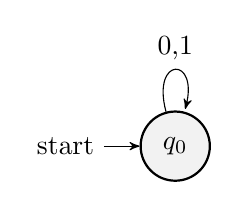
\begin{tikzpicture}
      \node[state, initial] (q0) {$q_{0}$};
      \draw (q0) edge[loop above] node{0,1} (q0);
    \end{tikzpicture}
  \end{center}
\end{node}

\begin{eg}
  The language $\Sigma^{*}$ is regular.
\end{eg}
\begin{node}
  This language is recognized by the following DFA:
  \begin{center}
    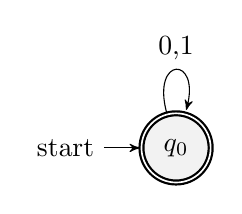
\begin{tikzpicture}
      \node[state, initial, accepting] (q0) {$q_{0}$};
      \draw (q0) edge[loop above] node{0,1} (q0);
    \end{tikzpicture}
  \end{center}
\end{node}

\begin{eg}\label{eg:finite-languages-regular}
  Every finite language $\Lfin$ is regular.
\end{eg}
\begin{node}
  The idea is that we can construct a DFA by brute force.
  This works because there are only finitely many strings in $\Lfin$, i.e., finitely many states suffice.
  For instance, suppose that $\Lfin = \Set{000, 010, 01}$.
  The following DFA recognizes $\Lfin$:
  \begin{center}
    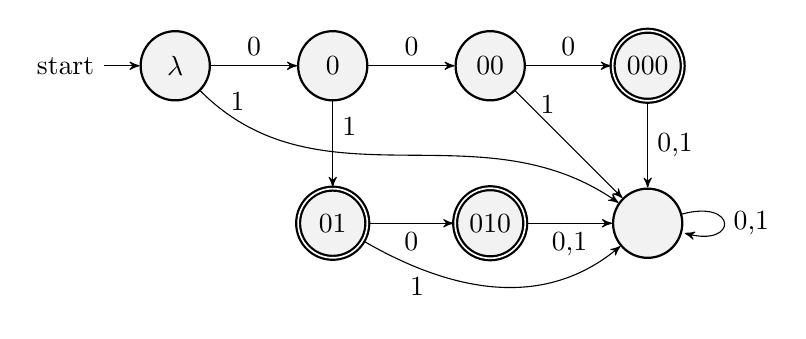
\begin{tikzpicture}
      \node[state, initial] (q0) {$\lambda$};
      \node[state, right of=q0] (0) {0};
      \node[state, right of=0] (00) {00};
      \node[state, accepting, below of=0] (01) {01};
      \node[state, accepting, right of=01] (010) {010};
      \node[state, accepting, right of=00] (000) {000};
      \node[state, right of=010] (dead) {};
      \draw (q0) edge node[above] {0} (0);
      \draw (q0) edge[out=-45, in=145] node[above, pos=0.1] {1} (dead);
      \draw (0) edge node[above] {0} (00);
      \draw (0) edge node[right, pos=0.3] {1} (01);
      \draw (00) edge node[above] {0} (000);
      \draw (00) edge node[above, pos=0.3] {1} (dead);
      \draw (000) edge node[right] {0,1} (dead);
      \draw (01) edge node[below] {0} (010);
      \draw (01) edge[out=-30, in=-140] node[below, pos=0.2] {1} (dead);
      \draw (010) edge node[below] {0,1} (dead);
      \draw (dead) edge[loop right] node[right] {0,1} (dead);
    \end{tikzpicture}
  \end{center}
\end{node}

\begin{defn}
  Let $L, L' \subseteq \Sigma^{*}$ be languages.
  The concatenation $L \cdot L'$ is the language
  $$
  L \cdot L' = \Set{s \cdot s' \in \Sigma^{*} \mid s \in L \wedge s' \in L'}
  $$
\end{defn}

\begin{thm}\label{thm:regular-closure}
  The class of regular languages is closed under intersection, union, complement, concatenation, and Kleene closure.
  That is, if $L$ and $L'$ are regular languages then so are $L \cap L'$, $L \cup L'$, $\Sigma^{*} \setminus L$, $L \cdot L'$, and $L^{*}$.
\end{thm}
\begin{proof}[Proof sketch]
  \begin{node}\label{node:tensor-of-dfa}%
    We only sketch the proof of closure under union.
    Let $D = (Q, \Sigma, \delta, q_{0}, F)$ (resp., $D' = (Q', \Sigma, \delta', q_{0}', F')$) be a DFA that recognizes $L$ (resp., $L'$).
    The main idea is to construct a new DFA that simulates both $D$ and $D'$:
    \begin{enumerate}
    \item take $Q \times Q'$ as the set of states;
    \item take $\Sigma$ as the alphabet;
    \item define the transition function $\Delta : (Q \times Q') \times \Sigma \to Q \times Q'$ by
      $$
      \Delta((q, q'), c) = (\delta(q, c), \delta'(q', c))
      $$
    \item take $(q_{0}, q_{0}') \in Q \times Q'$ as the initial state;
    \item take $\Set{(q, q') \in Q \times Q' \mid q \in F \vee q' \in F'}$ as the set of final states.
    \end{enumerate}
  \end{node}
\end{proof}

\section{Regular expressions}
\label{sec:regex}

\begin{defn}
  Given an alphabet $\Sigma$, \emph{regular expressions} are defined inductively as follows:
  \begin{enumerate}
  \item $\varnothing$ is a regular expression;
  \item $\varepsilon$ is a regular expression;
  \item each literal $c \in \Sigma$ is a regular expression;
  \item if $r$ and $r'$ are regular expressions then $r \cdot r'$ is a regular expression;
  \item if $r$ and $r'$ are regular expressions then $r + r'$ is a regular expression;
  \item if $r$ is a regular expression then $r^{*}$ is a regular expression.
  \end{enumerate}
\end{defn}

\begin{node}
  We have just defined the syntax of regular expressions.
  The semantics of regular expressions is defined by mapping each regular expression to a language.
\end{node}

\begin{defn}
  The language of a regular expression $r$ is defined by recursion on $r$:
  \begin{enumerate}
  \item the language of the regular expression $\varnothing$ is the empty language:
    $$\sL(\varnothing) = \varnothing$$
  \item the language of the regular expression $\varepsilon$ is the language containing just the empty string:
    $$\sL(\varepsilon) = \Set{\varepsilon}$$
  \item the language of the regular expression $c$ is the language containing just $c$: for each $c \in \Sigma$,
    $$\sL(c) = \Set{c}$$
  \item the language of the regular expression $rr'$ is the concatenation of $\sL(r)$ and $\sL(r')$:
    $$\sL(r \cdot r') = \sL(r) \cdot \sL(r')$$
  \item the language of the regular expression $r + r'$ is the union of $\sL(r)$ and $\sL(r')$:
    $$\sL(r + r') = \sL(r) \cup \sL(r')$$
  \item the language of the regular expression $r^{*}$ is the Kleene closure of $\sL(r)$:
    $$\sL(r^{*}) = (\sL(r))^{*}$$
  \end{enumerate}
\end{defn}

\begin{thm}\label{thm:regex-to-dfa}
  Let $e$ be a regular expression, $\sL(e)$ is regular, i.e., there is a DFA $D$ that recognizes $\sL(e)$.
\end{thm}
\begin{proof}
  \begin{node}
    We proceed by induction on the structure of $e$.
    When $e$ is $\varnothing, \varepsilon,$ or $c$, $\sL(e)$ is finite.
    In \cref{eg:finite-languages-regular}, we informally argued that finite languages are regular.
  \end{node}
  \begin{node}
    When $e$ is $r \cdot r'$ or $r + r'$, the induction hypothesis states that $\sL(r)$ and $\sL(r')$ are regular.
    By definition $\sL(r \cdot r') = \sL(r) \cdot \sL(r')$ and $\sL(r + r') = \sL(r) \cup \sL(r')$.
    By \cref{thm:regular-closure}, the class of regular languages is closed under concatenation and union, so $\sL(r \cdot r')$ and $\sL(r + r')$ are regular.
  \end{node}
  \begin{node}
    Finally, when $e$ is $r^{*}$, the induction hypothesis again states that $\sL(r)$ is regular.
    By definition, $\sL(r^{*}) = (\sL(r))^{*}$.
    By \cref{thm:regular-closure}, the class of regular languages is closed under Kleene closure, so $\sL(r^{*})$ is regular.
  \end{node}
\end{proof}

\begin{node}
  \cref{thm:regex-to-dfa} shows that every regular expression has a corresponding DFA.
  The converse is also true: every DFA has a corresponding regular expression.
  The proof of this fact is not trivial.
\end{node}

\end{document}